\SourceLeaf{202}4. \emph{Theorem.} Eine durch zwei im Planum $P$ liegende Punkte $T, U$
gezogene Gerade liegt ganz in jenem.

\textls{Beweis.} I) Liegt $A$ in der Geraden $\ldots TU \ldots$, so ist der Satz aus der
Definition des Planum von selbst klar. Liegt $A$ nicht in der Geraden $TU$, so
machen $AT$, $AU$ einen Winkel mit einander; ist nun

II) $AT = AU$, so folgt der Satz aus 3; sind hingegen

III) $AT$ und $AU$ ungleich, so sei $AT > AU$. Man verlängere $AT$ rückwärts
bis $AK = AT$; die Kreislinie, welche $T$ durch Drehung um $A$ beschreibt,
wird dann durch $K$ gehen, und die Kreisfläche, die ein Theil des Planum $P$
ist, wird durch $KT$ in zwei Theile getheilt, in deren einem $U$ liegt.

\begin{center}
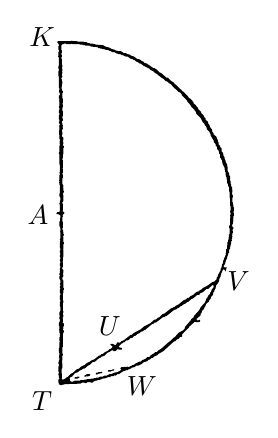
\begin{tikzpicture}[x=0.00633947cm,y=-0.00633947cm]
\fill[even odd rule] (112,44) -- (110,45) -- (84,45) -- (83,46) -- (83,48) -- (86,52) -- (86,54) -- (85,55) -- (85,62) -- (86,63) -- (86,66) -- (85,67) -- (85,74) -- (84,76) -- (86,78) -- (86,94) -- (85,95) -- (85,100) -- (86,101) -- (86,104) -- (85,105) -- (85,115) -- (86,116) -- (86,139) -- (87,140) -- (86,147) -- (88,150) -- (88,152) -- (86,155) -- (86,161) -- (87,162) -- (87,164) -- (86,165) -- (87,167) -- (87,175) -- (86,176) -- (86,178) -- (87,179) -- (87,183) -- (86,184) -- (86,189) -- (87,190) -- (87,193) -- (86,194) -- (86,202) -- (87,203) -- (87,206) -- (86,207) -- (86,209) -- (88,212) -- (88,213) -- (86,215) -- (87,217) -- (86,232) -- (87,233) -- (87,241) -- (88,242) -- (88,246) -- (87,247) -- (88,254) -- (87,255) -- (87,267) -- (86,268) -- (86,271) -- (87,272) -- (87,292) -- (88,293) -- (88,307) -- (87,308) -- (88,313) -- (87,314) -- (87,323) -- (86,324) -- (87,327) -- (86,329) -- (87,330) -- (87,333) -- (88,334) -- (88,350) -- (87,351) -- (87,356) -- (89,360) -- (89,364) -- (88,365) -- (88,369) -- (87,370) -- (87,372) -- (88,373) -- (88,386) -- (86,388) -- (83,388) -- (81,390) -- (81,391) -- (82,392) -- (85,392) -- (89,395) -- (88,406) -- (87,407) -- (87,416) -- (89,420) -- (89,426) -- (88,427) -- (89,429) -- (89,441) -- (88,442) -- (88,444) -- (89,445) -- (88,447) -- (88,460) -- (89,461) -- (89,464) -- (88,465) -- (88,470) -- (89,471) -- (89,473) -- (88,474) -- (88,478) -- (89,479) -- (89,482) -- (88,483) -- (88,486) -- (89,487) -- (89,490) -- (88,491) -- (88,496) -- (89,497) -- (89,499) -- (88,500) -- (88,510) -- (87,511) -- (87,514) -- (88,515) -- (87,517) -- (87,522) -- (89,525) -- (89,530) -- (88,531) -- (88,533) -- (89,534) -- (89,536) -- (88,537) -- (88,540) -- (89,541) -- (88,543) -- (88,550) -- (89,551) -- (89,554) -- (88,555) -- (88,564) -- (89,565) -- (89,567) -- (88,568) -- (88,577) -- (89,578) -- (89,586) -- (87,589) -- (87,595) -- (88,596) -- (87,598) -- (87,602) -- (88,603) -- (88,606) -- (86,610) -- (86,616) -- (87,617) -- (87,622) -- (86,624) -- (87,625) -- (87,630) -- (88,631) -- (88,638) -- (87,639) -- (87,646) -- (88,648) -- (87,649) -- (87,660) -- (86,661) -- (86,670) -- (87,671) -- (86,680) -- (87,681) -- (87,684) -- (86,685) -- (86,688) -- (85,689) -- (85,692) -- (86,693) -- (86,697) -- (85,698) -- (85,708) -- (86,709) -- (86,711) -- (85,712) -- (85,715) -- (86,716) -- (86,720) -- (87,721) -- (87,722) -- (85,724) -- (85,730) -- (86,731) -- (86,733) -- (89,735) -- (92,735) -- (93,734) -- (96,734) -- (97,733) -- (129,732) -- (132,730) -- (137,730) -- (138,731) -- (140,731) -- (143,729) -- (149,729) -- (150,730) -- (153,730) -- (156,727) -- (158,727) -- (159,726) -- (162,726) -- (163,725) -- (169,724) -- (173,722) -- (180,721) -- (184,719) -- (188,719) -- (190,717) -- (195,717) -- (197,715) -- (200,716) -- (203,713) -- (206,713) -- (215,707) -- (217,707) -- (221,705) -- (224,705) -- (226,703) -- (228,703) -- (232,700) -- (237,699) -- (241,696) -- (245,696) -- (251,693) -- (256,689) -- (263,687) -- (266,684) -- (268,684) -- (271,681) -- (273,681) -- (278,677) -- (283,675) -- (286,672) -- (295,667) -- (317,647) -- (319,647) -- (323,643) -- (326,642) -- (329,638) -- (332,638) -- (333,637) -- (333,633) -- (347,619) -- (347,618) -- (358,608) -- (361,608) -- (362,609) -- (368,608) -- (369,607) -- (369,605) -- (368,604) -- (366,605) -- (363,605) -- (362,604) -- (362,602) -- (370,595) -- (370,592) -- (372,590) -- (373,586) -- (377,582) -- (377,580) -- (379,578) -- (381,572) -- (387,567) -- (387,565) -- (390,562) -- (391,558) -- (394,555) -- (395,553) -- (395,550) -- (397,548) -- (398,544) -- (400,541) -- (401,535) -- (405,530) -- (407,526) -- (407,523) -- (410,517) -- (410,515) -- (411,514) -- (411,512) -- (414,505) -- (416,503) -- (417,503) -- (419,505) -- (419,507) -- (420,507) -- (422,500) -- (423,499) -- (418,499) -- (416,497) -- (416,496) -- (419,492) -- (421,484) -- (423,481) -- (423,478) -- (425,474) -- (425,471) -- (427,469) -- (427,464) -- (429,461) -- (429,457) -- (430,456) -- (430,453) -- (431,452) -- (431,447) -- (433,445) -- (432,442) -- (433,441) -- (433,438) -- (434,437) -- (433,434) -- (434,433) -- (434,430) -- (435,429) -- (434,423) -- (436,421) -- (436,419) -- (433,416) -- (433,414) -- (435,411) -- (435,407) -- (436,406) -- (435,402) -- (436,401) -- (436,396) -- (437,395) -- (437,390) -- (436,389) -- (436,387) -- (437,386) -- (437,379) -- (436,378) -- (436,374) -- (435,373) -- (435,369) -- (434,368) -- (434,359) -- (435,358) -- (435,355) -- (433,352) -- (434,344) -- (433,343) -- (433,338) -- (431,336) -- (431,332) -- (430,331) -- (430,326) -- (429,325) -- (429,316) -- (427,314) -- (427,310) -- (424,305) -- (424,297) -- (423,296) -- (423,292) -- (420,287) -- (420,285) -- (418,281) -- (418,278) -- (416,275) -- (415,269) -- (412,266) -- (412,260) -- (409,257) -- (409,255) -- (406,252) -- (406,248) -- (405,247) -- (404,242) -- (402,239) -- (402,237) -- (396,232) -- (396,230) -- (393,226) -- (393,222) -- (390,219) -- (387,212) -- (385,210) -- (385,207) -- (380,203) -- (380,200) -- (377,197) -- (376,194) -- (371,189) -- (371,187) -- (365,181) -- (365,179) -- (361,175) -- (361,174) -- (356,170) -- (356,168) -- (354,166) -- (354,165) -- (349,160) -- (348,160) -- (345,157) -- (345,156) -- (335,146) -- (334,146) -- (332,144) -- (331,142) -- (330,142) -- (320,132) -- (319,132) -- (316,128) -- (311,125) -- (304,118) -- (301,118) -- (291,109) -- (288,108) -- (282,102) -- (277,99) -- (275,99) -- (262,90) -- (258,89) -- (255,86) -- (252,85) -- (250,83) -- (246,81) -- (243,81) -- (238,77) -- (234,75) -- (232,75) -- (228,72) -- (223,71) -- (220,69) -- (216,69) -- (210,65) -- (204,65) -- (203,64) -- (200,64) -- (197,62) -- (192,61) -- (187,58) -- (179,56) -- (174,53) -- (159,52) -- (158,51) -- (155,51) -- (154,50) -- (148,50) -- (147,49) -- (144,49) -- (141,47) -- (136,47) -- (135,46) -- (123,46) -- (122,45) -- (113,45) -- cycle
(396,535) -- (396,539) -- (392,544) -- (391,548) -- (389,550) -- (389,552) -- (385,556) -- (384,559) -- (382,561) -- (379,569) -- (370,579) -- (367,585) -- (357,596) -- (356,599) -- (351,603) -- (351,604) -- (339,618) -- (338,622) -- (335,625) -- (326,630) -- (318,639) -- (317,639) -- (309,647) -- (308,647) -- (291,662) -- (286,665) -- (282,669) -- (279,669) -- (277,671) -- (270,675) -- (267,679) -- (263,679) -- (260,682) -- (253,685) -- (250,688) -- (247,688) -- (239,692) -- (237,694) -- (233,695) -- (231,697) -- (229,697) -- (226,699) -- (224,698) -- (211,699) -- (209,701) -- (209,702) -- (211,703) -- (211,704) -- (209,706) -- (203,709) -- (197,710) -- (191,713) -- (187,713) -- (186,714) -- (184,714) -- (182,716) -- (177,716) -- (174,718) -- (169,718) -- (165,720) -- (161,720) -- (160,721) -- (156,721) -- (155,722) -- (150,722) -- (149,723) -- (142,723) -- (141,724) -- (137,724) -- (136,725) -- (129,725) -- (128,726) -- (118,726) -- (114,728) -- (110,728) -- (108,726) -- (108,723) -- (107,721) -- (109,719) -- (112,718) -- (118,711) -- (124,709) -- (127,706) -- (130,705) -- (134,702) -- (137,702) -- (144,696) -- (148,694) -- (153,689) -- (158,688) -- (166,681) -- (168,681) -- (171,678) -- (177,676) -- (183,670) -- (188,668) -- (190,666) -- (194,665) -- (196,667) -- (199,667) -- (203,663) -- (205,663) -- (206,664) -- (211,664) -- (212,663) -- (212,661) -- (211,660) -- (208,660) -- (206,658) -- (206,657) -- (212,651) -- (213,651) -- (215,649) -- (217,649) -- (221,645) -- (224,645) -- (226,644) -- (230,640) -- (233,640) -- (237,636) -- (239,636) -- (244,632) -- (247,631) -- (250,628) -- (254,627) -- (256,625) -- (259,624) -- (272,613) -- (275,612) -- (277,610) -- (281,609) -- (294,599) -- (298,598) -- (300,596) -- (302,596) -- (317,584) -- (321,583) -- (323,581) -- (326,580) -- (329,577) -- (332,576) -- (334,574) -- (340,571) -- (343,568) -- (345,568) -- (348,565) -- (349,565) -- (352,562) -- (355,561) -- (362,555) -- (364,554) -- (367,554) -- (370,550) -- (374,549) -- (382,542) -- (385,542) -- (394,534) -- cycle
(127,719) -- (126,718) -- (123,718) -- (122,719) -- (118,719) -- (117,721) -- (118,722) -- (123,722) -- (124,721) -- (126,721) -- cycle
(137,718) -- (146,717) -- (148,716) -- (149,714) -- (148,713) -- (142,713) -- (137,716) -- cycle
(173,709) -- (171,708) -- (170,709) -- (165,709) -- (164,710) -- (161,710) -- (160,711) -- (160,713) -- (162,714) -- (165,712) -- (172,711) -- cycle
(197,704) -- (195,703) -- (191,705) -- (185,705) -- (184,707) -- (185,708) -- (189,708) -- (193,706) -- (196,706) -- cycle
(112,50) -- (113,51) -- (127,51) -- (128,52) -- (133,52) -- (134,53) -- (138,53) -- (139,54) -- (147,54) -- (151,56) -- (163,57) -- (165,59) -- (168,59) -- (169,60) -- (172,60) -- (173,61) -- (177,61) -- (178,62) -- (185,63) -- (186,64) -- (190,65) -- (192,67) -- (197,67) -- (202,70) -- (204,70) -- (205,71) -- (209,71) -- (212,73) -- (214,73) -- (220,76) -- (224,76) -- (229,80) -- (231,80) -- (232,81) -- (234,81) -- (236,83) -- (238,83) -- (241,86) -- (244,87) -- (248,90) -- (250,90) -- (255,94) -- (267,100) -- (270,103) -- (276,106) -- (279,109) -- (283,111) -- (287,115) -- (288,115) -- (291,118) -- (296,121) -- (300,125) -- (303,126) -- (309,131) -- (310,131) -- (318,140) -- (319,140) -- (326,147) -- (329,148) -- (331,150) -- (333,154) -- (342,163) -- (344,167) -- (348,171) -- (351,176) -- (358,183) -- (358,184) -- (361,187) -- (361,190) -- (370,199) -- (374,207) -- (378,211) -- (378,213) -- (381,216) -- (383,222) -- (387,226) -- (390,232) -- (390,234) -- (396,244) -- (397,248) -- (400,251) -- (400,254) -- (403,257) -- (403,261) -- (405,263) -- (407,267) -- (407,270) -- (409,272) -- (409,278) -- (411,280) -- (411,282) -- (413,284) -- (414,291) -- (418,299) -- (418,303) -- (419,304) -- (419,307) -- (420,308) -- (420,314) -- (421,315) -- (421,317) -- (422,318) -- (422,322) -- (423,323) -- (423,329) -- (425,332) -- (425,335) -- (427,338) -- (427,346) -- (428,347) -- (428,359) -- (429,360) -- (429,375) -- (430,376) -- (430,385) -- (429,386) -- (429,388) -- (430,389) -- (430,393) -- (429,394) -- (430,399) -- (429,400) -- (429,414) -- (427,416) -- (427,419) -- (428,420) -- (428,432) -- (427,433) -- (426,443) -- (425,444) -- (425,447) -- (424,448) -- (423,461) -- (421,463) -- (421,469) -- (420,470) -- (421,473) -- (420,474) -- (419,478) -- (417,480) -- (417,483) -- (415,486) -- (415,490) -- (413,493) -- (412,499) -- (410,502) -- (410,505) -- (405,514) -- (404,518) -- (402,520) -- (402,523) -- (398,527) -- (394,528) -- (383,536) -- (375,540) -- (371,544) -- (369,544) -- (366,547) -- (362,548) -- (355,554) -- (349,557) -- (346,560) -- (344,560) -- (339,564) -- (337,564) -- (326,573) -- (320,576) -- (318,578) -- (316,578) -- (314,580) -- (311,581) -- (298,591) -- (293,593) -- (287,599) -- (284,600) -- (281,603) -- (277,604) -- (269,611) -- (257,617) -- (250,623) -- (235,631) -- (232,634) -- (230,634) -- (216,645) -- (211,647) -- (208,650) -- (203,649) -- (201,653) -- (199,655) -- (193,652) -- (190,652) -- (189,654) -- (193,657) -- (193,659) -- (190,662) -- (187,663) -- (184,666) -- (178,669) -- (173,673) -- (171,673) -- (169,675) -- (166,676) -- (156,684) -- (154,684) -- (150,686) -- (148,688) -- (143,690) -- (138,694) -- (130,698) -- (126,702) -- (122,703) -- (113,711) -- (110,712) -- (103,719) -- (102,719) -- (97,723) -- (93,724) -- (91,722) -- (92,720) -- (91,703) -- (93,700) -- (93,692) -- (92,691) -- (93,679) -- (92,677) -- (94,675) -- (94,673) -- (93,672) -- (93,659) -- (94,658) -- (94,632) -- (96,628) -- (96,626) -- (94,624) -- (94,622) -- (95,621) -- (94,618) -- (96,616) -- (96,612) -- (93,609) -- (94,607) -- (94,602) -- (93,600) -- (95,597) -- (95,595) -- (94,594) -- (94,590) -- (95,589) -- (95,587) -- (94,586) -- (94,570) -- (95,569) -- (95,566) -- (94,565) -- (94,551) -- (95,550) -- (95,544) -- (96,543) -- (96,541) -- (95,540) -- (95,526) -- (93,523) -- (93,519) -- (95,516) -- (94,514) -- (95,505) -- (92,501) -- (94,497) -- (94,489) -- (93,488) -- (94,486) -- (94,479) -- (95,478) -- (95,464) -- (94,462) -- (95,461) -- (95,452) -- (96,451) -- (96,449) -- (95,448) -- (95,443) -- (94,442) -- (95,440) -- (94,436) -- (96,434) -- (96,433) -- (95,432) -- (94,424) -- (93,423) -- (93,420) -- (94,419) -- (94,408) -- (93,407) -- (93,398) -- (94,396) -- (93,394) -- (97,390) -- (97,389) -- (93,386) -- (94,384) -- (94,372) -- (93,371) -- (93,368) -- (95,365) -- (95,362) -- (94,361) -- (95,359) -- (95,354) -- (94,353) -- (94,351) -- (96,347) -- (95,345) -- (95,340) -- (94,339) -- (95,335) -- (93,332) -- (93,320) -- (94,319) -- (94,313) -- (93,312) -- (93,310) -- (94,309) -- (94,302) -- (93,301) -- (94,299) -- (94,284) -- (93,283) -- (93,280) -- (94,279) -- (94,272) -- (95,271) -- (95,259) -- (96,258) -- (96,256) -- (94,254) -- (94,252) -- (95,251) -- (95,249) -- (94,248) -- (95,239) -- (92,236) -- (92,233) -- (93,232) -- (93,227) -- (92,226) -- (92,223) -- (94,221) -- (94,219) -- (93,218) -- (94,214) -- (93,213) -- (93,210) -- (92,209) -- (92,206) -- (94,204) -- (94,201) -- (93,200) -- (93,196) -- (94,195) -- (94,186) -- (93,185) -- (93,178) -- (94,177) -- (94,173) -- (93,172) -- (93,170) -- (94,169) -- (94,161) -- (93,160) -- (93,156) -- (92,154) -- (93,153) -- (93,149) -- (94,148) -- (94,146) -- (92,144) -- (92,142) -- (91,141) -- (92,131) -- (93,130) -- (93,126) -- (92,125) -- (92,122) -- (91,121) -- (91,119) -- (93,116) -- (92,114) -- (92,110) -- (93,109) -- (93,107) -- (92,106) -- (93,104) -- (92,97) -- (93,96) -- (93,93) -- (92,92) -- (92,81) -- (91,80) -- (91,77) -- (92,76) -- (92,73) -- (91,72) -- (91,69) -- (92,68) -- (92,64) -- (91,63) -- (91,53) -- (93,51) -- (95,51) -- (96,50) -- (100,50) -- (101,51) -- (110,51) -- cycle;
\node[inner sep=0pt] at (52,37) {$K$};
\node[inner sep=0pt] at (44,394) {$A$};
\node[inner sep=0pt] at (446,527) {$V$};
\node[inner sep=0pt] at (188,617) {$U$};
\node[inner sep=0pt] at (252,736) {$W$};
\node[inner sep=0pt] at (52,766) {$T$};
\end{tikzpicture}

\end{center}

Indem nun eine Gerade $TK$ sich so bewegt, dass ihr einer Endpunkt in $T$, der
andere in der Peripherie $KVW$ bleibt, beschreibt sie das Planum, vollendet
die Figur immer vollkommener und hat sie ganz erschöpft, wenn $W$ in $T$
angekommen ist. In einer Lage der beweglichen Geraden ist sie also durch $U$
gegangen, es sei diess die Lage $TV$. Die Gerade $TU$ ist also nur ein Theil
der Geraden $TV$, letztere aber liegt ganz in der Ebene, dasselbe gilt also
auch von $TU$.



Dass übrigens auf vorbeschriebene Art die Fläche des Halbkreises ganz
ausgefüllt wird, kann leicht mit vollkommener Strenge bewiesen werden.
Gesetzt Ein Theil könne nicht erreicht werden und $U$ sei ein Punkt in
demselben. Mit einem Radius kleiner als $TU$ beschreibe man [um $T$] eine
Kugelfläche, wodurch jener Halbkreis in die Theile $M$, $M'$ getheilt wird,
so dass $M$ ausserhalb, $M'$ innerhalb der Kugelfläche liege; offenbar ist
dann $U$ in $M$. Es sei ferner $W$ der Punkt der Peripherie des Halbkreises,
wo dieselbe von der Kugelfläche geschnitten wird; die gerade Linie $TW$ liegt
dann innerhalb $M'$, also $U$ innerhalb der Figur $KTWK$, diese aber wird
beschrieben, indem die bewegliche Linie sich von der Lage $TK$ bis zu der
Lage $TW$ dreht. Also ist die Voraussetzung, dass $U$ nicht getroffen werde,
absurd.

